We hebben in onze buis met ballen ervaren dat we wat kracht moeten zetten om de ballen erin te krijgen. De kracht die nodig was hebben we de spanning genoemd, maar we hebben niet verklaard waarom er kracht nodig is om de extra bal erin te krijgen. De reden is de weerstand.

Als we de + en de - van een batterij met elkaar verbinden dat maken we een kortsluiting. Bij een kortsluiting gaat er heel veel stroom lopen, zoveel zelfs dat het plastic om de geleider in brand zou kunnen vliegen. Om te voorkomen dat dat gebeurt moeten we de stroom beperken. Dit doen we door de weerstand\index{Weerstand} te verhogen. De weerstand vermindert de stroom.

Er zijn verschillende manieren om de weerstand te verhogen. We kunnen gebruik maken van een apparaat in de stroomkring, zoals een schoepenrad in de rivier. Een schoepenrad in de rivier verbruikt het water niet, maar zorgt er wel voor dat de rivier minder hard stroomt. Zo zal ook een gebruiker in de stroomkring (bijvoorbeeld een lamp die brandt) er voor zorgen dat de weerstand verhoogd wordt. In de elektronica gebruiken hebben we ook speciale componenten me de naam weerstand\index{Weerstand}\index{Resistor} die we kunnen opnemen in een stroomkring. De enige functie van de weerstand in een circuit is het verhogen van de totale weerstand zodat de stroom beperkt wordt.

In de elektronica wordt een weerstand weergegeven met het symbool dat je ziet weergegeven in \ref{symbool:weerstand}

\begin{figure}[h]
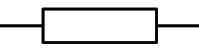
\includegraphics[width=5cm]{weerstand}
\centering
\caption{Symbool van een weerstand}
\label{symbool:weerstand}
\end{figure}


